\documentclass[11pt,reqno]{amsart}
\usepackage{geometry}                % See geometry.pdf to learn the layout options. There are lots.
\geometry{letterpaper}                   % ... or a4paper or a5paper or ... 
%\geometry{landscape}                % Activate for for rotated page geometry
\usepackage[parfill]{parskip}    % Activate to begin paragraphs with an empty line rather than an indent
\usepackage{graphicx}
\usepackage{amssymb}
%\usepackage{epstopdf}
\usepackage{url}
%\DeclareGraphicsRule{.tif}{png}{.png}{`convert #1 `dirname #1`/`basename #1 .tif`.png}
\usepackage{amsfonts}
\usepackage{amsmath}
%\usepackage{xspace}
%\usepackage{hyperref}
%\usepackage{algorithm}
%\usepackage{algorithmic}
%\usepackage{graphicx}
%\usepackage{algorithm}
%\usepackage{algorithmic}
%\usepackage{amssymb}
%\usepackage{caption}
%\usepackage{subcaption}
\usepackage{listings}
\usepackage{color}
\usepackage{balance}

\newif\ifanswers

% uncomment if you want answers to appear
%\answerstrue
% uncomment if you want answers to be suppressed
\answersfalse

\definecolor{darkgreen}{rgb}{0,.4,0}
\definecolor{orange}{rgb}{.8,.4,0}
\lstset{ 
  language=Lisp, 
  basicstyle=\small\ttfamily, 
  keywordstyle={}, 
  %commentstyle=\em \color{green}, 
  %frame=L,
  %float=tbph,
 % captionpos=b,
  showstringspaces=false, 
  keywordstyle=[3]\bf\color{orange},
  keywords=[3]{<>},
  keywordstyle=[2]\bf\color{darkgreen},
  keywords=[2]{predict,observe,assume,observe-csv},
  mathescape=true,
  stringstyle={},
           } 
\renewcommand*{\lstlistingname}{Program}

\lstnewenvironment{bodycode}[2]{\small\lstset{caption=#1,label=#2,basicstyle=\small\ttfamily}}{}
%\lstnewenvironment{code}[1][]{\lstset{caption=#1,label=#1}}{}
\lstnewenvironment{code}[2]{\small\lstset{caption=#1,label=#2}}{}

\newcommand{\+}[1]{\ensuremath{{\mathbf{#1}}}}

\newenvironment{inline}[1]{{\small\ttfamily #1}}{}

\renewcommand\vdots{%
  \vbox{\baselineskip2pt\lineskiplimit0pt\kern1pt\hbox{.}\hbox{.}\hbox{.}\kern-1pt}}

\newcommand{\bx}{{\bf x}}

\newcommand{\bz}{{\bf z}}

\title{Writing a Rejection Sampler}
\author{Frank Wood, Brooks Paige}
%\date{}                                           % Activate to display a given date or no date



\begin{document}
\maketitle
%\section{}
%\subsection{}


{\bf Introduction}
%\vspace{.5cm}

In this exercise we will write a rejection sampler which draws from a Poisson distribution.
\begin{figure}[tb]
\centering
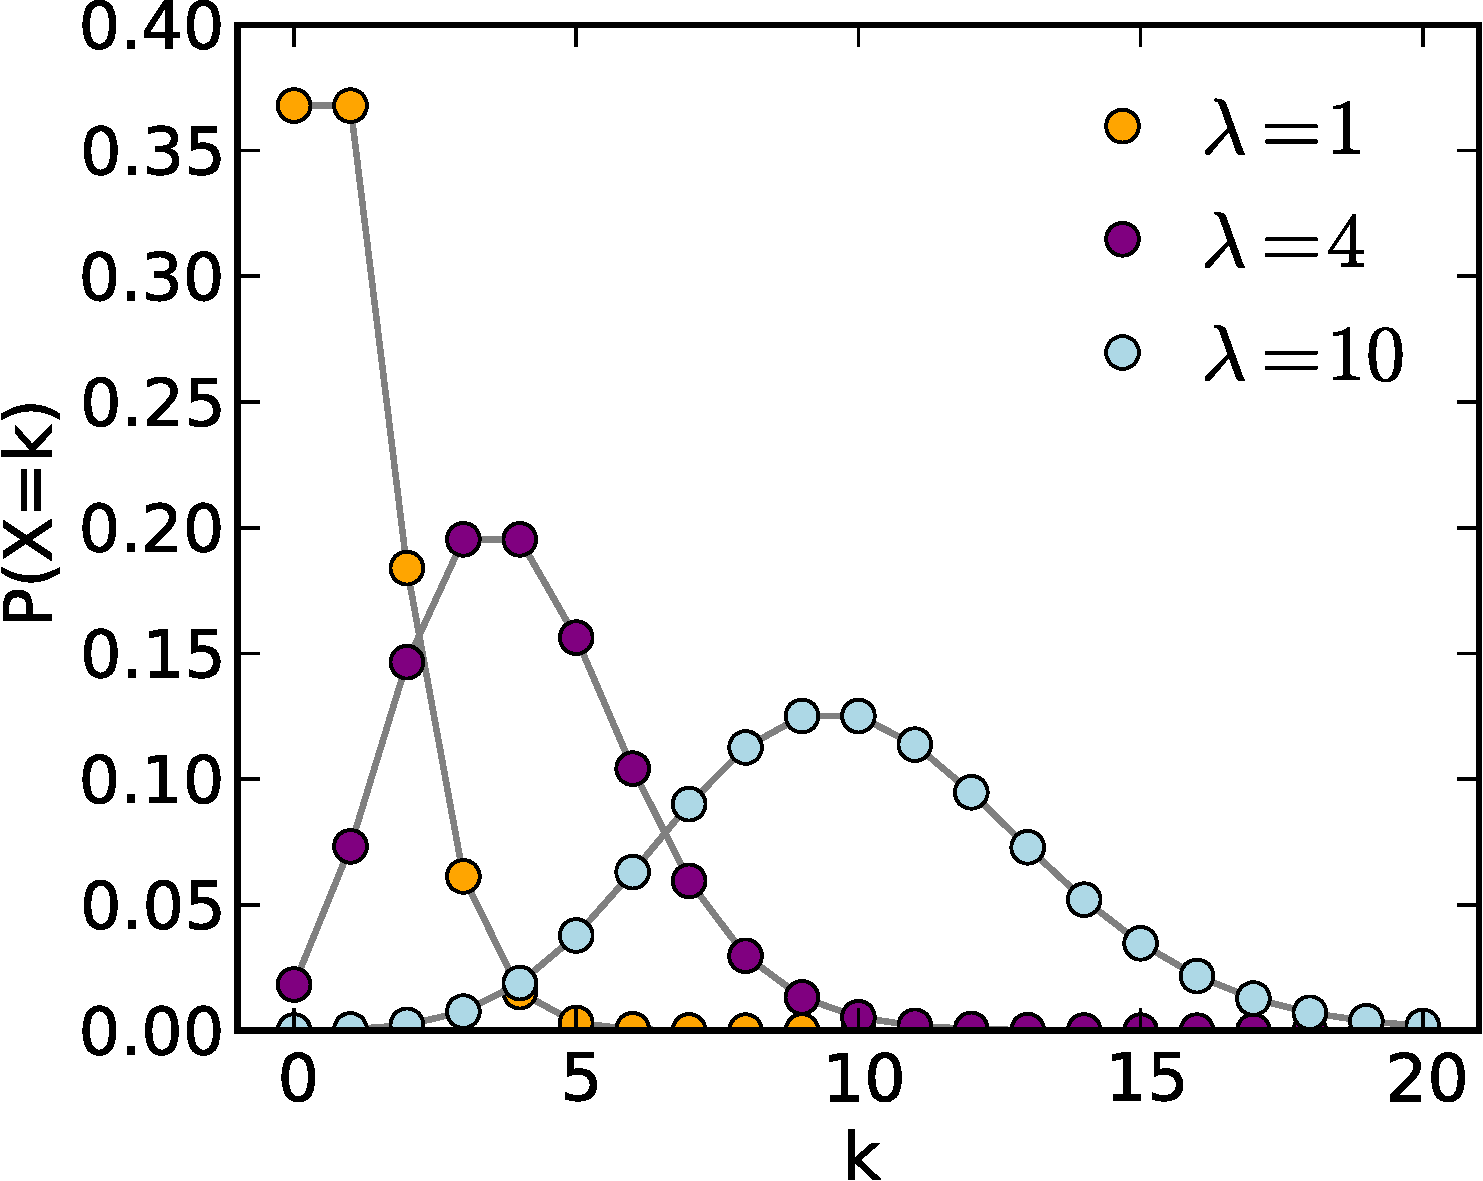
\includegraphics[width=0.4\textwidth]{poisson-pmf}
\caption{The probability mass function for a Poisson distributed random variable. 
Figure from Wikipedia: \inline{http://en.wikipedia.org/wiki/Poisson\_distribution}.
}
\end{figure}
An algorithm to sample a Poisson random variate $k$ with rate $\lambda$ is given by \cite{knuth1969}.
Initialize $L \leftarrow e^{-\lambda}$, $k \leftarrow 0$, and $p \leftarrow 1$, and then loop:
\begin{enumerate}
\item Update $k \leftarrow k+1$
\item Sample $u \sim \mathrm{Uniform}(0, 1)$
\item Update $p \leftarrow p \times u$
\item If $p \le L$ return $k -1$; otherwise repeat.
\end{enumerate}
This algorithm increments $k$ until eventually returning.

Note that each run of the program generates an execution trace with a possibly different amount of randomness;
that is, sampling a value of $k=10$ requires more random choices than a value of $k = 5$.
If $\lambda = 4$, then under a Poisson distribution the probability masses $p(k=3) = p(k=4)$, but in this algorithm generating a $k = 4$ variate requires more random choices.

Particularly vexing, each random choice is a draw from Uniform$(0, 1)$, meaning that if we label all the random choices $u_1, \dots, u_k$, then for each $u_i$ we have $p(u_i) = 1$.

\begin{figure}[tb]
\centering
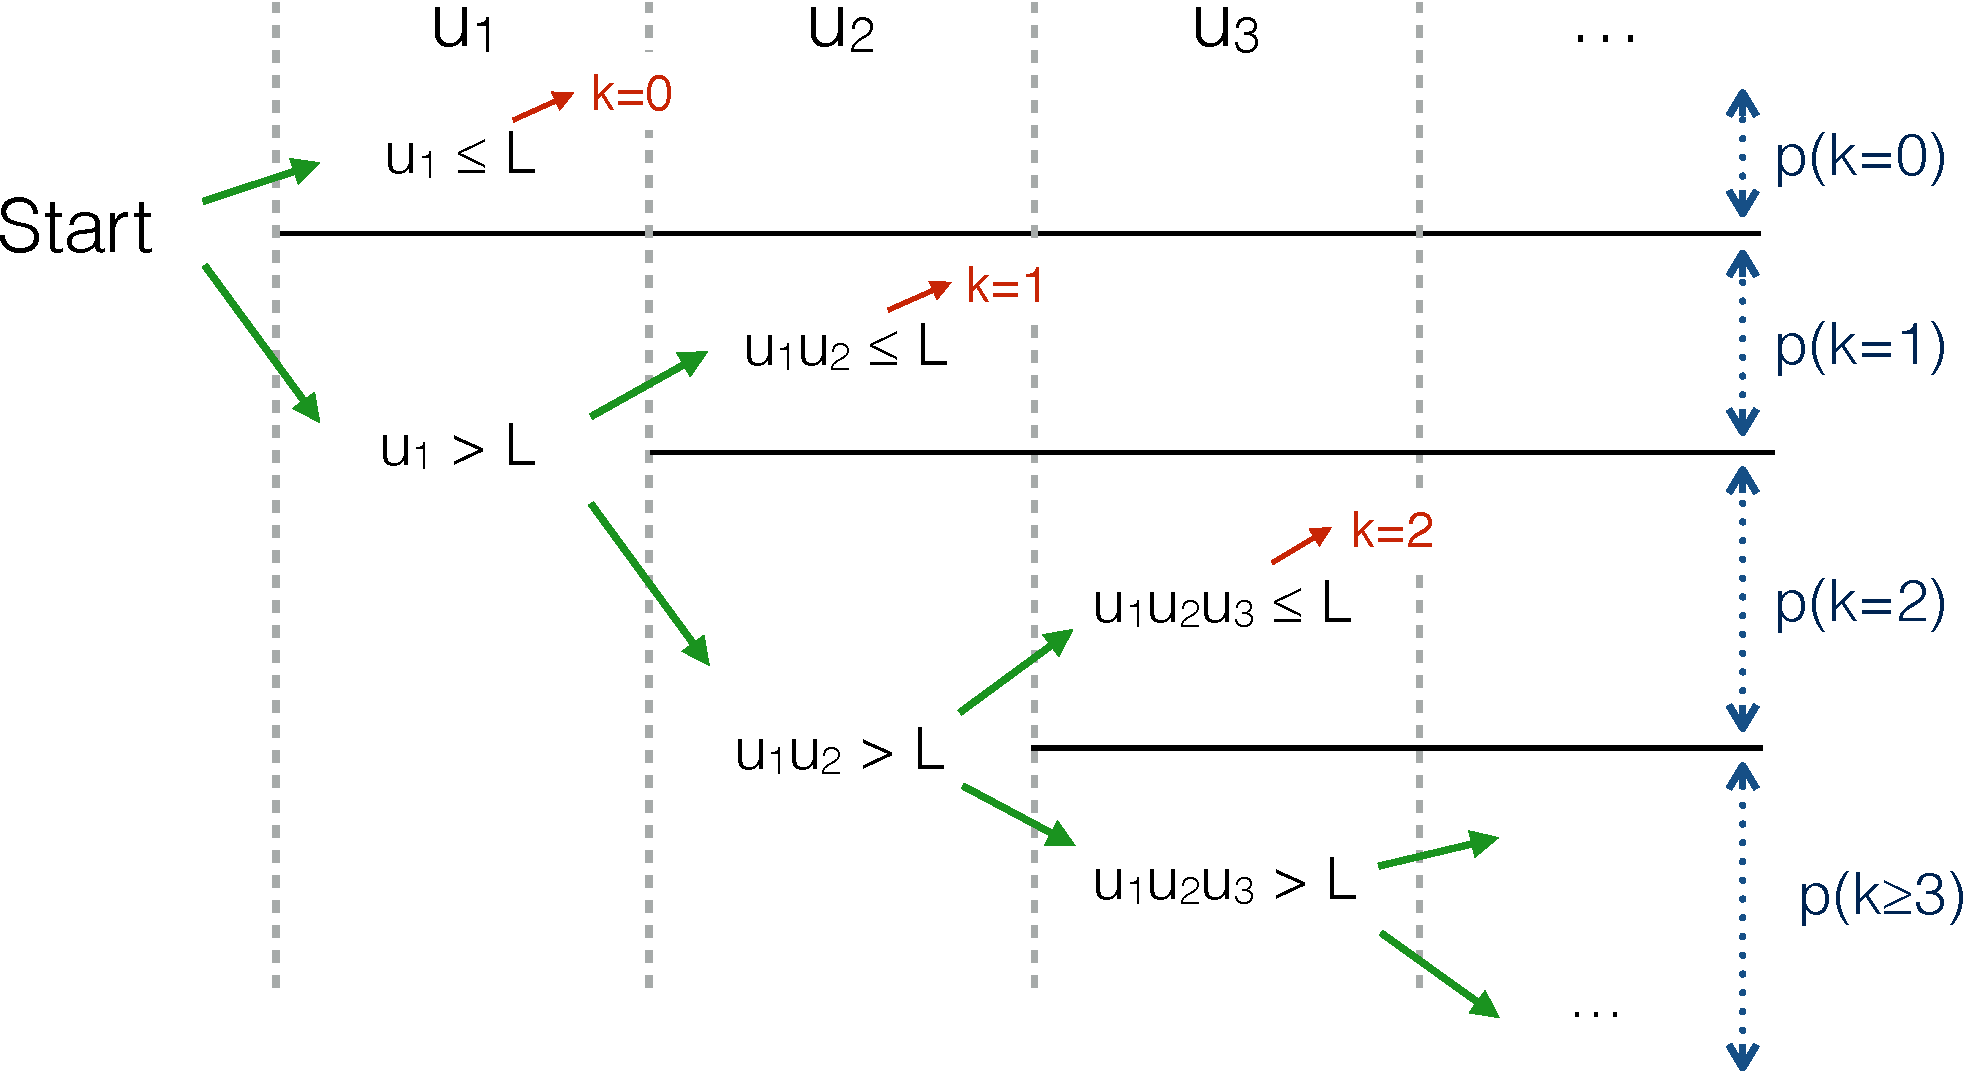
\includegraphics[width=\textwidth]{execution-diagram-crop}
\caption{Diagram showing sequential steps during the execution of the sampler program.
Execution flows to the right; each column shows a random draw $u_i \sim \mathrm{Uniform}(0, 1)$.
Green arrows represent the program branching that occurs at the end of each algorithm iteration.
Red arrows denote program termination, with a given return value of $k$.}
\label{fig:exec}
\end{figure}

The execution path of this program is shown in Figure~\ref{fig:exec}.
Since the probability of the program execution trace is defined as the product of the probabilities of all random choices made in the execution of the program \cite{Wood-AISTATS-2014,Paige-ICML-2014},
then each execution of the program has the same probability, regardless of $k$, with
\begin{align}
p(\mathrm{trace}) &= \prod_{i=1}^k p(u_i) = 1
\end{align}
for all $k = 0, 1, 2, \dots$.
The probability of sampling a particular value $k$ is directly related to the length of the program execution trace ---
the algorithm is defined in such a way that, although each individual execution trace has equal probability, the number of execution traces which terminate after $k$ total uniform draws is proportional to a Poisson distribution with rate $\lambda$.
%For example, suppose $\lambda = 4$. 
%The probability of the algorithm terminating after 3 random choices $u_1, u_2, u_3$ and then returning a sample $k = 2$ is given by the Poisson mass function
%\begin{align}
%p(k=2|\lambda=4) = \frac{4^2e^{-4} }{2!} \approx 0.1465.
%\end{align}

We can compute the probability of this program halting (i.e.~returning a value) after any particular number of random choices $n$ have been made.
Letting $L \equiv e^{-\lambda}$, we can compute these probabilities, for example
\begin{align}
p(\mathrm{halt}=1) &= p(u_1 \le L) = L = e^{-\lambda}
%\mathrm{Bernoulli}(L) \\
\end{align}
which is exactly the probability that $k = 0$ under a Poisson distribution.
We can compute this for higher numbers of random variables as well, although it becomes cumbersome:
\begin{align}
p(\mathrm{halt}=2) &= p(u_1u_2 \le L, u_1 > L) \\
&=  p(u_2 \le \frac{L}{u_1}, u_1> L) \\
&= \int_{u_1=L}^1 \frac{L}{u_1} du_1 \\
&= -L \log L = \lambda e^{-\lambda},
\end{align}
which matches the Poisson mass $p(k=1|\lambda)$, and
\begin{align}
p(\mathrm{halt}=3) &= p(u_1u_2u_3 \le L, u_1 > L, u_2 > \frac{L}{u_1}) \\
&=  p(u_3 \le \frac{L}{u_1u_2}, u_1> L, u_2>\frac{L}{u_1}) \\
&= \int_{u_1=L}^1 \int_{u_2=L/u_1}^1 \frac{L}{u_1u_2} du_2du_1 \\
&= L \int_{u_1=L}^1 \frac{1}{u_1} \int_{u_2=L/u_1}^1 \frac{1}{u_2} du_2du_1 \\
&= L \int_{u_1=L}^1 \frac{-\log (L/u_1)}{u_1} du_1 \\
&= L \int_{u_1=L}^1 \frac{\log(u_1) - \log(L)}{u_1} du_1 \\
&= L \left [ \int_{u_1=L}^1 \frac{\log(u_1)}{u_1} du_1 - \log(L) \int_{u_1=L}^1 \frac{1}{u_1} du_1 \right ] \\
&= L \left [\frac{-(\log L)^2}{2} + (\log L)^2 \right ] \\
&= L \frac{(\log L)^2}{2} = e^{-\lambda} \frac{\lambda^2}{2}
%&= -L \int_{u_1=L}^1 \frac{\log u_1}{u_1} du_1 \\
%&= - \frac{L(\log L)^3}{2} = \frac{\lambda^3}{2} e^{-\lambda}
\end{align}
which matches the Poisson mass $p(k=2|\lambda)$, and so on.

\pagebreak
{\bf Questions:}

{\bf (1)} Write this sampler by filling in the missing function marked \inline{<$\cdots$>} in the following program:
\begin{code}{}{}
[assume sample-poisson (lambda (rate) (begin
    (define L (exp (* -1 rate)))
    (define inner-loop (lambda (k p)
    	<$\cdots$>
    ))
    (inner-loop 1 (uniform-continuous 0 1))))]
    
[predict (sample-poisson 4)]
\end{code}
Confirm this function actually generates Poisson random variates.

\ifanswers
\begin{quotation}
{\bf Answer:}
\begin{code}{}{}
[assume sample-poisson (lambda (rate) (begin
    (define L (exp (* -1 rate)))
    (define inner-loop (lambda (k p)
        (if (<= p L)
            (dec k)
            (begin
                (define u (uniform-continuous 0 1))
                (inner-loop (inc k) (* p u))))))
    (inner-loop 1 (uniform-continuous 0 1))))]
    
[predict (sample-poisson 4)]
\end{code}
\end{quotation}
\fi

{\bf (2)} 
Review the two sampling approaches --- particle Gibbs and random database --- described in sections 3.1 and 3.2 of \cite{Wood-AISTATS-2014}\footnote{http://jmlr.org/proceedings/papers/v33/wood14.pdf}.
Although no posterior inference is being performed in this example, the two methods differ considerably in the manner by which consecutive samples are drawn.
It is important to realize that for either approach, executing the program generates a {\em dependent} chain of Poisson random variates.

%In the particle MCMC approach, each individual sweep outputs $L$ particles.
%There is a weak dependence between sweeps, as a single sample ($\+x^\star$ in Algorithm~1 of \cite{Wood-AISTATS-2014}) is retained from one sweep to the next,
%but given that each proposed particle is drawn by an execution the \inline{sample-poisson} algorithm it is unsurprising that the output has the correct distribution.

In random db, an initial sample is drawn by running the program forward once.
Subsequent samples are proposed by 
\begin{enumerate}
\item selecting an individual random choice $u_i$ from the uniform draws $u_1, \dots, u_{k+1}$ instantiated in the current sample;
\item resampling a program suffix beginning from $u_i$, by drawing a new value $u_i'$, forgetting all random choices $u_{i+1}, \dots, u_{k+1}$, and continuing program execution from the point at which $u_i$ is drawn; this will create a new sequence of random choices $u_i', \dots, u_{k'+1}'$ where $k$ and $k'$ are not necessarily the same;
\item accepting or rejecting the new proposed set of random choices with probability given by Equation~5 in \cite{Wood-AISTATS-2014}.
\end{enumerate}
Assuming running \inline{sample-poisson} generates an independent sample from a Poisson distribution, show that the random db algorithm over this program defines a Markov chain whose stationary distribution is the same Poisson.

\ifanswers
\begin{quotation}
{\bf Answer: }
For this program, we can significantly simplify the expression for Eq.~5 in \cite{Wood-AISTATS-2014}.
First, since there are no \inline{observe} statements in this program, note that $p(\+y|\+x) = p(\+y|\+x') = 1$. 
Since all draws over the course of program execution are from a Uniform(0,1) density, we have $p(\+x) = p(\+x') = 1$ and
$p(\+x\setminus\+x'|\+x\cap\+x') = p(\+x'\setminus\+x|\+x'\cap\+x) = 1$.
Thus we have an acceptance probability $A(k \rightarrow k')$ of
\begin{align}
p(\mathrm{accept}) &= \min \left ( 1, 
\frac{ p(\+y|\+x') p(\+x') |\+x| p(\+x\setminus\+x'|\+x\cap\+x') }{p(\+y|\+x) p(\+x) |\+x'| p(\+x'\setminus\+x|\+x'\cap\+x) } 
\right ) \\
A(k \rightarrow k') &= \min \left ( 1, \frac{k+1}{k'+1} \right ).
\label{eq:ratio}
\end{align}
Now, consider the proposals themselves; given a particular $k$, we propose $k'$ by continuing the Poisson sampler routine starting from some fixed point $i$.
Suppose $Y$ is a Poisson random variable, with density $f(Y)$ and distribution function $F(Y)$.
Consider a conditional Poisson density $p(Y=k' | k' \ge i-1)$ for $i \ge 1$,
\begin{align}
p(Y=k' | k' \ge i-1) &= \frac{p(Y=k', k' \ge i-1)}{p(k' \ge i-1)}
\\
&=
\frac{f(Y=k')\mathbb{I}_{[k' \ge i-1]}}{\int_{j = i-1}^\infty f(Y=j) dY}
\\
&=
\frac{f(Y=k')\mathbb{I}_{[k' \ge i-1]}}{\int_{j = 0}^\infty f(Y=j) dY - \int_{j = 0}^{i-1} f(Y=j) dY}
\\
&=
\frac{f(Y=k')\mathbb{I}_{[k' \ge i-1]}}{1 - F(i-1)}.
\end{align}
Since $i$ is proposed uniformly from $1, \dots, k+1$, we can write out the proposal kernel $g(k \rightarrow k')$ which is implicitly used by random db to propose a new value $k'$ given a current value $k$, by marginalizing over the choice of $i$:
\begin{align}
g(k \rightarrow  k') &= \sum_{i=1}^{k+1} p(Y=k' | k' \ge i-1)p(i | k) \\
&= \frac{f(Y=k')}{k+1} \sum_{j=0}^{k} \frac{\mathbb{I}_{[k' \ge j]}}{1 - F(j)}.
\label{eq:proposal}
\end{align}
So, random database works by proposing new values from the kernel $g(k \rightarrow k')$ in Eq.~\ref{eq:proposal}, and accepting it with probability $A(k \rightarrow k')$ in Eq.~\ref{eq:ratio}.
Combining these, the overall transition probability $p(k \rightarrow k')$
is defined as 
\begin{align}
p(k \rightarrow k') &= g(k \rightarrow k')A(k \rightarrow k').
\label{eq:transition}
\end{align}
This transition probability can be written as a product of the density $f(\cdot)$ in the numerator of Eq.~\ref{eq:proposal} and a piecewise-defined function $h(k, k')$, by considering the different cases in which $k$ or $k'$ is the greater value:
\begin{align}
p(k\rightarrow k') &= f(Y=k')h(k, k'),
\label{eq:transition-factored}
\\ %&
\nonumber \\
%\end{align}
%where we define $g(k, k')$ as
%\begin{align}
h(k, k') &=
\begin{cases}
\dfrac{1}{k'+1} \sum_{j=0}^{k} \dfrac{1}{1 - F(j)} &\mbox{if } k < k' \\
\dfrac{1}{k+1} \sum_{j=0}^{k} \dfrac{1}{1 - F(j)} &\mbox{if } k = k' \\
\dfrac{1}{k+1} \sum_{j=0}^{k'} \dfrac{1}{1 - F(j)} &\mbox{if } k > k'.
\end{cases}
\end{align}
Note that the function $h(\cdot)$ is symmetric in its arguments; that is, $h(k, k') = h(k', k)$.
\vspace{1em}

\noindent To confirm that the stationary distribution of this operator is Poisson (i.e.~has density $f(Y)$), we check that it satisfies the detailed balance equation
\begin{align}
f(k')p(k' \rightarrow k) = f(k)p(k \rightarrow k').
\end{align}
Substituting our expression in Eq.~\ref{eq:transition-factored} above, we have
\begin{align}
f(Y=k')f(Y=k)h(k', k) &= f(Y=k)f(Y=k')h(k, k').
\end{align}
Since $h(k, k') = h(k', k)$, these quantities are equal and detailed balance holds, so $f(Y)$ is indeed the stationary distribution of $p(k \rightarrow k')$, and thus the Markov chain of samples generated by random db are appropriately Poisson distributed.
\end{quotation}
\fi

\bibliographystyle{plain}
\bibliography{../refs}




\end{document}  